\subsection{Построение Roren graph-a}

Отдельная вершина, в которую происходит трансляция roren transform-ов - это wrapper или обертка. Рассматриваемая обертка должна хранить в себе информацию о положении в исходном графе, тип transform-а, входные и выходные collection-ы.

Из wrapper-ов построена иерархия. Существует единый интерфейс обертки, который частично реализуют гранулярный wrapper и графовый wrapper (рис~\ref{fig:iwrapper}). Логически гранулярный wrapper - это набор некоторых Part-ов, которые в себе сохраняют информацию о преобразовании, его входных и выходных коллекциях. В свою очередь, графовый wrapper хранит уникальный идентификатор вершины и глубину слоя в графе.

\begin{figure}[h]
    \centering
    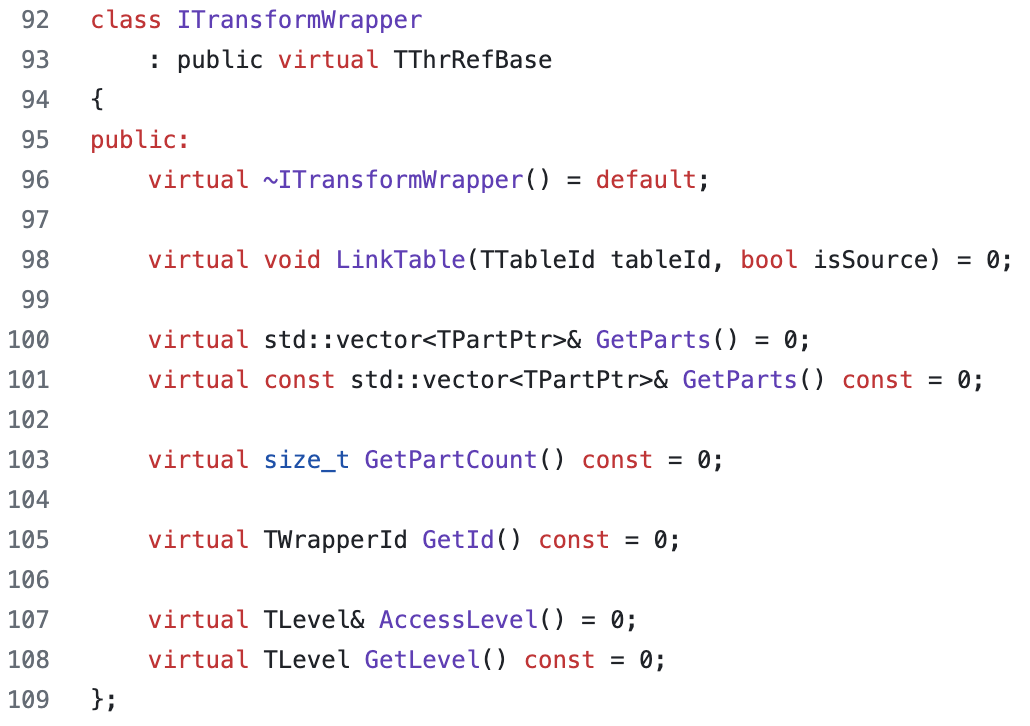
\includegraphics[width=\textwidth]{img/iwrapper.png}
    \caption{Интерфейс обертки для конденсации}
    \label{fig:iwrapper}
\end{figure}

Далее по иерархии в соответствие с transform-ами из API Roren сопоставлены wrapper: ReadWrapper, WriteWrapper, ParDoWrapper, GroupByKeyWrapper и FlattenWrapper.

У ParDoWrapper-а есть возможность сколлапсировать с другим ParDoWrapper-ом. Это естественная возможность, т.к. логически ParDo является фукнцией над некоторыми входными данными, а коллапсирование - способ выразить композицию функций. Однако помимо объединения в композицию функций из двух функций с разными входами можно сделать одну с многими входными таблицами.

Здесь важно заметить, что практически каждый wrapper может иметь входные или выходные таблицы, кроме GroupByKeyWrapper и FlattenWrapper. Очевидно, что ReadWrapper и WriteWrapper имеют какие-то входные и выходные таблицы соответственно. Ради упрощения конденсации графа, ParDo Wrapper в отличие от ParDo может иметь входные и выходные таблицы, как результат слияния с ReadWrapper или WriteWrapper.
